\documentclass{article}
\usepackage[utf8]{inputenc}
\usepackage{clrscode3e}
\usepackage[english]{babel}
\usepackage{blindtext}
 \usepackage{graphicx}
 \usepackage{hyperref}
 \hypersetup{
    colorlinks=true,
    linkcolor=blue,
    filecolor=magenta,      
    urlcolor=cyan,
}
\urlstyle{same}
\pagestyle{plain}
\begin{document}

\graphicspath{ {./images/} } 
\begin{titlepage}
 
   \begin{center}
   
       \vspace*{1cm}
       \Huge
       \textbf{Grid Path}

     
            
       \vspace{1 cm}
      \LARGE
       \textbf{Buzdug\u{a} Ionu\c{t} Gabriel}\\
       Group 1.1B\\
       Year 1\\
       Computer Science
       \vfill
            
      
            
       \vspace{0.8cm}
      
    
    \end{center}
  \end{titlepage}
\newpage

\section {\LARGE Problem Statement} \vspace*{1cm}
\LARGE \textbf{Grid Path} \vspace*{1cm}
\par Consider a field in form of a squared grid of nxn dimensions.
Each location of the grid is defined by a positive integer which represents 
the elevation(height of a point of the field projected on a  horizontal reference plane).
\par Find a path from the leftmost top corner to the corner of the field located in the bottom right
such that:
\par i)Movement along the field can only be made down or to the right.
\par ii)The cost of the path,calculated as the sum of the absolute values of the difference between to consecutive
locations along the path is minimum.
Two algorithms will be implemented.
\newpage
\section {\LARGE Pseudocode}
\Large \par In this section there are presented the two algorithms used for solving the problem.
\begin{enumerate}
  \item The first Algorithm uses a recursive aproach which is a fairly trivial solution to the problem.Because the same sub-problems are going to be 
  solved multiple times,the time complexity is will be exponential,
  $\Theta (2^n)$.For every cell there are two options.

  \item The second algorithm uses Dynamic programming by creating an aditional 
  matrix in which each element stored holds the value of the minimum cost path
  up until that element.\par After the matrix is filled,we can start printing the 
  path starting from the top left corner and choosing the minimum value of the 
  two moves we are allowed to make,going right or down.The time complexity for
  this algorithm is the size of the matrix,$\Theta(n^2)$.
  
\end{enumerate}
\par To simplify the Pseudocode appeareance,the names of some variables were shortened: 
\begin{itemize}
  \item $matrix \Rightarrow A $
  \item $row\_ index \Rightarrow i $
  \item $col\_ index \Rightarrow j $
  \item $MinCost \Rightarrow B $
  \item The abso(\textbf{int} a,\textbf{int} b) function which returns the absolute value between two variables is also included in the pseudocode.
\end{itemize}

\subsection{Recursive Algorithm Pseudocode}
\Large
\begin{codebox}
\Procname{$\proc{FindPathRec}(A,i,j)$}
\li     \If $i \isequal 0$   and  $j \isequal 0$\li      \Then   \Return $0$        
\End
\li     \If $i \isequal 0$ \li     
\Then   \Return $\proc{FindPathRec}(A,i,j-1)+abso(A[i][j-1],A[i][j])$         
\End
\li     \If $j \isequal 0$ \li     
\Then   \Return $\proc{FindPathRec}(A,i-1,j)+abso(A[i-1][j],A[i][j])$          
\End
\li
$a \gets \proc{FindPathRec}(A,i-1,j)+abso(A[i-1][j],A[i][j]) $
\li
$b \gets \proc{FindPathRec}(A,i,j-1)+abso(A[i][j-1],A[i][j]) $
\li     \If $a <  b$ \li     
\Then   \Return $a$ \li
        \Else \li \Return $b$ 
\End


\end{codebox}
 \vspace*{1cm}
\par This is the first part of the recursive aproach.\par The FindPathRec function 
returns the minimum cost path for a single location.To be able to print all the
locations we also need the printalg1 function.
\newpage
\begin{codebox}\Procname{$\proc{printalg1}(A)$}
\li $i \gets 0$
\li $j \gets 0$
\li Print the top left location of the path
\li
\While $i \le $\attrib{A}{no\_rows}-1$ $ and $j \le $\attrib{A}{no\_cols}-1$ $\Do\li
 \If $i \isequal $\attrib{A}{no\_rows}-1$ $  and  $j \isequal $\attrib{A}{no\_cols}-1$ $      \Then \li break\End
 \li\If $j \isequal $\attrib{A}{no\_cols}-1$  $ 
 \Then \li $i \gets i+1$\li Print Current location  
 \li \ElseIf $i \isequal $\attrib{A}{no\_rows}-1$ $ \Then \li 
 $ j \gets j+1$ \li Print Current location
 \li \ElseIf $ \proc{FindPathRec}(A,i+1,j) <  \proc{FindPathRec}(A,i,j+1) $ \Then \li 
 $ i \gets i+1$ \li Print Current location\li 
 \Else \Then \li $ j \gets j+1$ \li Print Current location
 
\end{codebox}
\par This function  prints all the elements of the path by calling the FindPathRec function in a succesive way starting from the top left corner of the grid to the bottom left one .
\\
\par On the next page we have the Dynamic Programming pseudocode for implementing the algorithm.
\subsection{Dynamic Programming aproach}
\newpage


\begin{codebox}\Procname{$\proc{FindPathDP}(A)$}
\li \For $i\gets 1 $ \To $\attrib{A}{no\_rows}-1$
\li \Do $B[i][0] \gets B[i-1][0]+abso(A[i-1][0],A[i][0])$
\li $B[0][i] \gets B[0][i-1]+abso(A[0][i-1],A[i][0])$ \End
\li \For $i\gets 1 $ \To $\attrib{A}{no\_rows}-1$
\li \Do \For $j\gets 1 $ \To $\attrib{A}{no\_cols}-1$ \Do
\li  $ m \gets B[i-1][j]+abso(A[i-1][j],A[i][j])  $
\li  $ n \gets B[i][j-1]+abso(A[i][j-1],A[i][j])  $
\li \If $m<n$ \Then \li
$B[i][j] \gets m$
\li \Else  \li $B[i][j]=n$ \End \End \End
\li $i \gets 0$
\li $j \gets 0$
\li Print the top left Location
\li
\While $i \le $\attrib{A}{no\_rows}-1$ $ and $j \le $\attrib{A}{no\_cols}-1$ $\Do\li
 \If $i \isequal $\attrib{A}{no\_rows}-1$ $  and  $j \isequal $\attrib{A}{no-cols}-1$ $      \Then \li break\End
 \li\If $j \isequal $\attrib{A}{no\_cols}-1$  $ 
 \Then \li $i \gets i+1$\li Print Current location  
 \li \ElseIf $i \isequal $\attrib{A}{no\_rows}-1$ $ \Then \li 
 $ j \gets j+1$ \li Print Current location
 \li \ElseIf $ B[i+1][j] <  B[i][j+1] $ \Then \li 
 $ i \gets i+1$ \li Print Current location\li 
 \Else \Then \li $ j \gets j+1$ \li Print Current location
\end{codebox}
\newpage
\par In this graph we can see the comparison of the time complexity of the two algorithms
\begin{figure}[h]
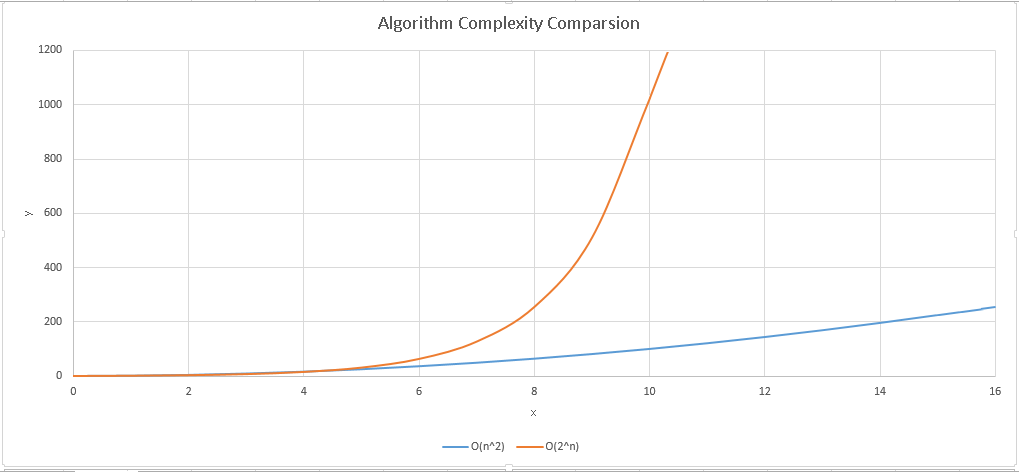
\includegraphics[width=12 cm, height=10cm]{graph}
\end{figure}
\newpage
\section{Experimental data}
\Large
\vspace*{1cm}
\par In this section it is presented how the experimental values are generated
for our problem.
\par To create our grid we need to randomly generate a matrix of dimension nxn.
     The dimension of the matrix is going to be a randomly generated integer 
     represented by the variable $matrix.no\_rows$.
\par Then we can generate the elements of the grid which have random values
between $[0,10000]$.
\par Because the recursive algorithm has an exponential time complexity,generating
values for both algorithms comes in with a few restrictions.In that case, to avoid
getting high time consuming experimental data for the recursive algorithm,we are going to create a matrix that has a dimension of maximum 10x10.
\par The second algorithm will be run on the same set of values as the first one 
so we can have a comparsion of running time,but also it will run on a separate set
of data that is much larger.
\par Even then,a restriction of a matrix of a maximum dimension of 300x300 needs to be made because we need to make sure that the file in which we put the experimental values doesn't get too large.
\par This is essential for testing the algorithms side by side but also for testing 
on non trivial sets of data.
\newpage
\section{Experimental Application Structure}
\subsection{High Level Application Structure}
\par In this section we review the modular structure of our application on a high level hierarchy. 
\begin{figure}[h]
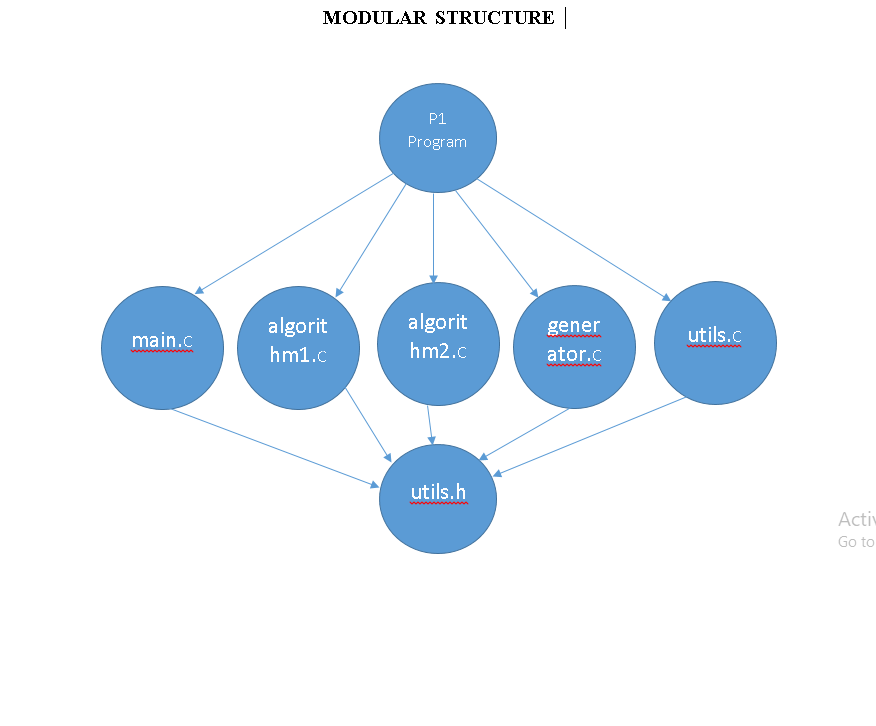
\includegraphics[width=12 cm, height=10cm]{structure}
\end{figure}
\par Our program uses a modular structure so that it can be easily divided 
in different work files.
\par All the ".c" files are part of the project structure and are interconnected by the use utils.h in which all the functions used in the project are located. 
\newpage
\subsection{Description of input data}
\par Our input data is relevant to what the algorithm needs to work and is composed
from multiple data sets which contain:
 \begin{itemize}
     \item The dimension of the grid represented 
    \\ by $matrix.no\_rows$ 
    \\$1 \le $matrix.no\_rows$ \le 10 $ Used for the comparison of both types of algorithms
    \\$1 \le $matrix.no\_rows$ \le 300 $ Used for the Dynamic Programming algorithm
     \item $matrix.no\_rows^2$ elements which represent the value of each location 
     of the grid.
     \\Each element is represented by \\$0 \le matrix[row\_index][col\_index] \le 10000$
   \end{itemize}
\subsection{Description of output data/results}
\par In the results section it is presented how the output data sets of the problem
are being made.
\par Each one of the two algorithms outputs the minimum cost path,starting from the top left corner
of the matrix to the bottom right one.
\par Each location of the path is printed in order as  $Mincost[row\_index][col\_index]$.
\par In the end a row/multiple rows of such locations are printed on the terminal.
\par As a method of ease when reading the result a restriction has been implemented
for grids with many elements.Only the first and last 10 locations are printed,the other values being replaced by three dots "...".
\newpage
\subsection{List of Application modules}
\begin{enumerate}
  \item The algorithm1.c module
  \par Here we have implemented the first algorithm using the recursive aproach.
  \par The module consists of two functions:
  \begin{itemize}
  \item FindPathRec (which computes the minimum \\path up to a certain element)
  \item printalg1 (which calls the first function in order to print all the minimum cost locations.
\end{itemize}
  \item The algorithm2.c module
  \par In this module we have implemented the second algorithm based on the Dynamic Programming aproach.
  \par The module consists of one function:
  \begin{itemize}
  \item FindPathDP (which computes prints the minimum \\path of the grid).
  
\end{itemize}
  \item The generator.c module
  \par This is the module used for the generation of data sets.
  \par The module consists of one function:
  \begin{itemize}
  \item $create\_ematrix$ (which generates a matrix \\with random elements and dimension).\\It also puts the data sets in a file for use \\in the python implementaion.\\
  The functions for both of the algorithms are\\ called here as well on different data sets.
\end{itemize}
\newpage
\item The utils.c module
\par In this module there are multiple utility functions used in the implementation of the application.
\item The main.c module
\par This the main function in which the other modules are called.
\par main.c also contains a switch function which is used for easy access of other modules and convenience in comparing the two algorithms as many times as the user wants.
\item The utils.h header
\par In this module we have the headers for all the functions used in the application ,the file utils.h being included in all the other .c extension files.
\end{enumerate}
\newpage 
\subsection{List of all procedures/functions used in the application}
\begin{enumerate}
    \item algorithm1.c
   \begin{itemize}
       \item \textbf{int} FindPathRec\\(struct $grid\_matrix$ matrix,int $row\_index,$int $ col\_index$)\\
       This function is used for the recursive algorithm.
       \par It computes the minimum cost necesarry to reach a certain location.The function works its way back the grid calculating each time what is the\\ minimum sum of absolute values to location A[0][0].
       The path it can take is limited by two moves up and to the left.
       \par If the current location calculated is either on the first row of the matrix or on the first column it will have only one path to take so it will go straight to the first element.\\
       \textbf {Parameters:}
       
       \begin{itemize}
           \item The first parameter is \textbf{struct $grid\_matrix$ matrix}
           \\This is the matrix which holds the randomly generated values.
           It has a struct form so we can easily allocate values and free the matrix.
           \item The second parameter is \textbf {int $row\_index$}
           \\It holds the row of the location.
           \item The third parameter is \textbf {int $row\_column$}
           \\It holds the column position of the location.
       \end{itemize}
        \par The function returns the minimum cost value up until the location defined by the row and column indexes.
    \newpage
    \item \textbf{void} printalg1(struct $grid\_matrix$ matrix)
    \par The role of this function is to start printing the locations of the
    shortest path on the grid.
    \par It starts with the first location of the grid and then check to see which of the two options:going to the right or down has the minimum cost value.
    \par If it reaches the last column or last row it will only count one of those two directions.
    \par The function stops once it reaches the bottom right location. 
   \end{itemize} 
  \item algorithm2.c
  \par This module only contains one funtion:
  \begin{itemize}
      \item int FindPathDP(struct $grid\_matrix$ matrix)
      \par This function represents the second algorithm implemented and it uses a Dynamic Programming aproach.
     \par The difference between this function and the last one is that
     we use a newly created matrix\\(MinCost) to save the minimum cost path to each location.
     \par This way we don't have to call the function for each element
     when printing.The printing procedure stays the same,only we start from the first element of the new matrix and search the minimum path possible.
     \\
     \par The only parameter used is the randomly generated matrix which is used to create the new one.
    
  \end{itemize}
  \newpage
  \item generator.c
  \par This module contains only one function which has two roles:
  \begin{itemize}
      \item Creating a randomly generated matrix
      \item Executing the two algorithms on this particular set of data.
  \end{itemize}
  \par The function \textbf{void} $create\_matrix$(\textbf{int} $grid\_dimension$) has only one parameter. 
  \par This parameter determines if the geneator creates a matrix of maximum dimension of 10x10 or a one with a maximum of 300x300.
  \par These sets of data are relevant for comparing the two algorithms
  as the first one can give a decent running time only if the matrix dimension is around 10x10.
  \par So depending on what algorithm we want to show this function is going to call the other two functions from algorithm1.c and algoritm2.c
  \item utils.c
  \par This module is where our utility functions are located.
  \begin{itemize}
      \item The first function is:
      \\\textbf{int} min(\textbf {int} a,\textbf{int} b)
      \par It returns the minimum value between the two parameters.
      \par This function is used while finding the minimum of two consecutive locations.
      \newpage
      \item The second function is:
      \\\textbf{int} abso(\textbf {int} a,\textbf{int} b)
      \par It returns the absolute value between two elements.
      \par This function is used to get the absolute value between two consecutive locations.
      \item The third function is:
      \\\textbf{void} $set\_value$ which has 4 parameters:
      \begin{itemize}
          \item \textbf{struct} $grid\_matrix$ matrix
          \item \textbf{int} $row\_index$
          \item \textbf{int} $columm\_index$
          \item \textbf{int} $element\_value$
      \end{itemize}
      \par This function is used to set the value of each element in the matrix.
      \item The fourth function is:
      \\\textbf{void} $get\_value$ which has 3 parameters:
      \begin{itemize}
          \item \textbf{struct} $grid\_matrix$ matrix
          \item \textbf{int} $row\_index$
          \item \textbf{int} $columm\_index$
      \end{itemize}
      \par This function is used to get the value of each element in the matrix.
      \item The last function in this module is:
      \\\textbf{void} $print\_matrix$(\textbf{struct} $grid\_matrix$ matrix)
      \par This function has only one parameter,a matrix of type struct.
      \par The role of this function is to print the values in the text file.
      
  \end{itemize}
  \item utils.h -Contains all the headers for the functions from above
  
\end{enumerate}
\newpage
\subsection{Results and Conclusions}
\par In this section we will conduct two sets of tests to evaluate how out algorithms differ in running time.
\begin{enumerate}
\item The first test will be made on 10 different data sets comparing the two algorithms in both C and Python language.

\begin{figure}[h]
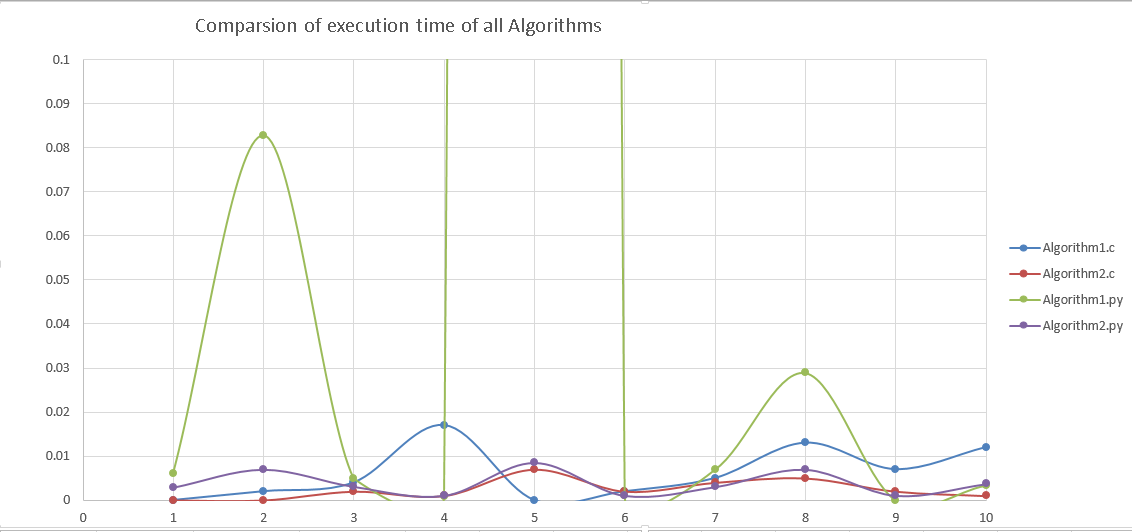
\includegraphics[width=12 cm, height=10cm]{graph2}
\end{figure}
\par On three of the algorithms the results are very similar.
\par One massive difference is on the Algorithm1.py.
\par We can already see that the first algorithm has a higher running time even on the C implementation,and when impemented in python the differences are even higher.
\newpage
\begin{figure}[h]
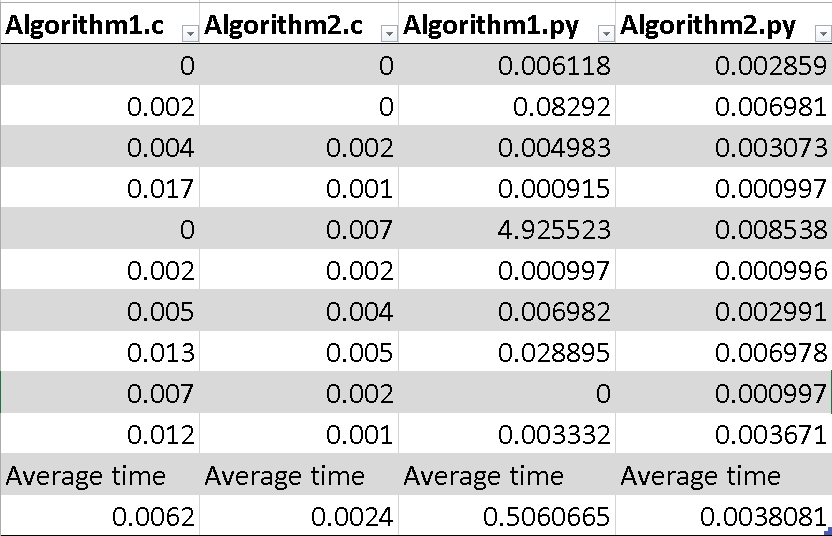
\includegraphics[width=10cm, height=10cm]{table}
\end{figure}
\par Here is the table of results.
\par We can see that the fifth set of data in python is way higher than the rest.
\par The average time of each implementation is also shown,the dynamic programming algorithm implemented \\in C(Algorithm2.c) having the best running time average. 
\par \textbf{The main part} about these sets of data is that they were run on a matrix of a maximum dimension of 10x10 because,otherwise the first algorithm would take too long to run because it has a exponential running time.
\newpage 
\item
\par The second set of tests will be made on a larger matrix,but the 
results will only be computed for the implementations of the second algorithm.
\begin{figure}[h]
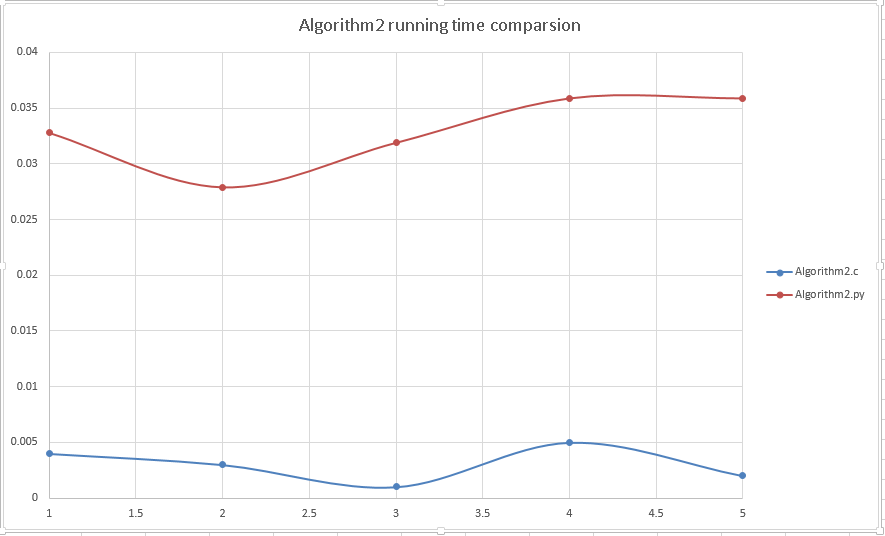
\includegraphics[width=10cm, height=10cm]{graphalg2}
\end{figure}
\par In this graph we can see how the Dynamic Programming algorithm(Alogrithm2) runs in both C and Python.
\par the algorithm implemented in C is much faster than the one in python.
\par The diffence in running time comes from the fact the Python is an interpreted language,where as C is a compiled language.
\newpage
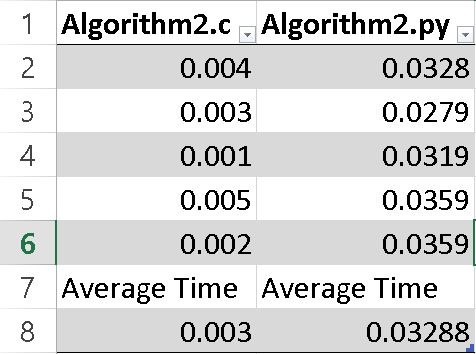
\includegraphics[width=10cm, height=10cm]{tablealg2}
\par In this table we can see what values we got from using 5 data sets.
\par The average time on the algorithm implemented in C is much lower than
the algorithm implemented in python.
\\
\par \textbf{Conclusions}
\par After implementing both algorithms and comparing them in both C and Python language we can tell the differences and draw conclusions.
\par Most importantly is how much time the algorithms take to run.
\newpage
\par In this case, it was a challenging task to compare the two algorithms,because of how they behave on large sets of data.

\par Due to how the Recursive algorithm has an exponential running time 
it was hard to compare on a matrix that is larger than 10x10.
\par Regarding this problem,I chose to review both algorithms on a smaller scale,and show only how the Dynamic Programming algorithm behaves on sets of bigger matrices.
\par After the tests,results showed that even though all the algorithms produce the same output values,the Dynamic programming algorithm implemented in C language has the fastest running time.
\subsection {References}
\begin{enumerate}
\item \href{https://www.geeksforgeeks.org/}{GeeksforGeeks.com}
\item \href{https://stackoverflow.com/}{StackOverflow.com}
\item \href{https://en.wikipedia.org/wiki/Dynamic_programming/}{Dynamic Programming-Wiki}
\end{enumerate}
\end{enumerate}
\end{document}


